\section{Esperimento di Stern e Gerlach} %Esperimento di Stern e Gerlach
Considero un sistema di particelle con momento angolare di spin 1/2, in moto lungo y, soggette ad un campo magnetico con un gradiente lungo la direzione z.
\begin{center}
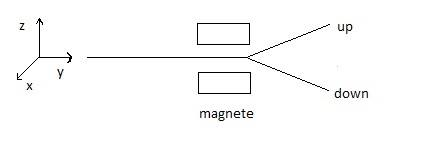
\includegraphics[scale=0.5]{immagini/stern-gerlach.jpg} %immagine
\end{center}

Il gradiente produce una forza traslazionale che direziona le particelle verso l'alto o verso il basso, a seconda che lo spin sia rispettivamente up o down. \\
I due autovalori dell'energia corrispondenti ai due gradi di libertà di spin, sono
\begin{equation}\begin{split}
E_{\pm}=\pm\gamma(B_{0}+\alpha z)\frac{\hbar}{2}
\end{split}\end{equation}
con $\gamma>0$ rapporto giromagnetico  e  $\alpha$ gradiente lungo z.\\
Prese le particelle in un particolare stato iniziale, le collimiamo selezionando quelle con un valore preciso della velocità; queste particelle le preparo poi in uno stato di sovrapposizione di spin up e spin down:
\begin{equation}\begin{split}
c_{\uparrow}\left|\uparrow\right\rangle+c_{\downarrow}\left|\downarrow\right\rangle
\end{split}\end{equation}
dove, per la condizione di normalizzazione risulta
\begin{equation}\begin{split}
\left|c_{\uparrow}\right|^2 = p
\end{split}\end{equation}
\begin{equation}\begin{split}
\left|c_{\downarrow}\right|^2 = 1-p
\end{split}\end{equation}
Il sistema considerato presenta due gradi di libertà per particella: la coordinata x (dipendente dal tempo) che però non è rilevante ai fini della nostra indagine perché abbiamo preparato le particelle in modo che traslino con velocità costante; e il tempo di nostro interesse.\\
Dopo un tempo di volo T, le particelle si raggruppano in due macchie distinte e simmetriche rispetto alla direzione di volo.\\
Consideriamo una particella nello stato iniziale
\begin{equation}\begin{split}
\left|z_{0}\right\rangle (c_{\uparrow}\left|\uparrow\right\rangle+c_{\downarrow}\left|\downarrow\right\rangle)
\end{split}\end{equation}
applichiamo l'Hamiltoniana (che supponiamo agire per un dato periodo) e ne facciamo la rappresentazione z\\
\begin{equation}\begin{split}
\left\langle z\right| \exp (-\frac{itH}{\bar{h}})\left|z_{0}\right\rangle (c_{\uparrow}\left|\uparrow\right\rangle+c_{\downarrow}\left|\downarrow\right\rangle)=\\
\textrm{sostituendo gli autovalori}\\
=c_{\uparrow}\exp(i \gamma T B_{0}\frac{1}{2}) \left|\uparrow\right\rangle \exp(i \alpha \gamma \frac{T}{2}z)+ c_{\downarrow}\exp(-i \gamma T B_{0}\frac{1}{2}) \left|\downarrow\right\rangle \exp(-i \alpha \gamma \frac{T}{2}z)=\\
=c_{\uparrow}\left|\uparrow\right\rangle \left|1\right\rangle_{ORB} + c_{\downarrow}\left|\downarrow\right\rangle \left|2\right\rangle_{ORB}
\end{split}\end{equation}
dove $\left|\uparrow\right\rangle$ e $\left|\downarrow\right\rangle$ rappresentano lo stato di spin e $\left|1\right\rangle$ e $\left|2\right\rangle$ lo stato orbitale.\\
Da questa descrizione si sa che:
\begin{itemize}
\item se preparo una particella in uno stato up $\left|\uparrow\right\rangle$ (ponendo $c_{\uparrow}=1$ e $c_{\downarrow}=0$)\\la ritrovo nello stato up $\left|\uparrow\right\rangle \left|1\right\rangle_{ORB}$;
\item se preparo una particella in uno stato down $\left|\downarrow\right\rangle$ (ponendo $c_{\uparrow}=0$ e $c_{\downarrow}=1$)\\la ritrovo nello stato down $\left|\downarrow\right\rangle \left|2\right\rangle_{ORB}$;
\item se invece preparo le particelle in una sovrapposizione ottengo uno stato entangled.
\end{itemize}
\subsection{Interpretazione}
Il termine $\left|c_{\uparrow}\right|^2$ rappresenta la probabilità di trovare la particella nello stato up
il termine $\left|c_{\downarrow}\right|^2$ rappresenta la probabilità di trovare la particella nello stato down. Se preparo le particelle in una sovrapposizione, esse saranno in due differenti autostati della posizione, non sono in una mistura tra stato up e stato down ma in uno stato entangled.

\section{Gatto di Schrödinger} %Gatto di Schrödinger
Schrödinger propose un paradosso con il quale riuscì a enfatizzare il problema concettuale emerso nell'esperimento di Stern e Gerlach:

Un gatto viene messo in una stanza con pareti metalliche insieme con il seguente congegno infernale [...] All'interno di un contatore Geiger c'è una piccolissima quantità di sostanza radioattiva, così piccola che c'è un'uguale probabilità che in un'ora decada uno degli atomi o che non ne decada nessuno. Se uno decade, allora il contatore scatta e tramite un relè attiva un martelletto che rompe una fiala contenente cianuro. Se si prepara tutto il sistema e si aspetta un'ora, si può dire che il gatto è vivo se non è decaduto nessun atomo ed è morto se è decaduto anche solo un atomo.

La sostanza radioattiva si trova in uno stato di sovrapposizione: decaduta - non decaduta.
\begin{itemize}
\item Se la sostanza non decade il gatto è vivo cioè siamo in uno stato $\left|\psi_{vivo}\right\rangle$;
\item Se la sostanza decade il gatto è morto cioè siamo in uno stato $\left|\psi_{morto}\right\rangle$;
\item Se faccio una sovrapposizione (partendo con il gatto vivo)
\begin{equation}\begin{split}\begin{split}
(c_{\uparrow}\left|\uparrow\right\rangle + c_{\downarrow}\left|\downarrow\right\rangle)\left|\psi_{vivo}\right\rangle=\\
=c_{\uparrow}\left|\uparrow\right\rangle\left|\psi_{vivo}\right\rangle + c_{\downarrow}\left|\downarrow\right\rangle\left|\psi_{morto}\right\rangle
\end{split}\end{split}\end{equation}
ottengo uno stato entangled nel quale il gatto non è né vivo né morto.
\end{itemize}

Si crea un problema concettuale: se vedo la particella in un posto ben preciso, essa dovrebbe essere in un autostato della posizione ben preciso (cioè il gatto dove essere vivo o morto) non può essere entangled.

\section{Von Neumann} %Von Neumann
Von Neumann interviene in questa descrizione affermando che nella misura interferisce anche la nostra mente: quando io guardo il gatto la mia mente risulta in uno stato entangled con la convinzione che il gatto sia vivo quando la particella non è decaduta, e con la convinzione che il gatto sia morto quando la particella è decaduta.\\
Von Neumann sostiene che in questa catena ci debba essere qualcosa, alla fine, che deve collassare; questo è necessario affinché sia verificato il postulato di Von Neumann, cioè se il risultato è su si deve trovare nell'autostato su, mentre se il risultato è giu si deve trovare nell'autostato giù.\\
Questo collasso viene nel cervello, cioè lo creo io quando decido il risultato, che è un dato obiettivo e quindi associato ad uno stato preciso.
Il problema è che se collassa un elemento della catena collassa tutto.

Consideriamo lo stato
\begin{equation}\begin{split}
\frac{1}{2}(\left|\uparrow\right\rangle \left|1\right\rangle + \left|\downarrow\right\rangle \left|2\right\rangle)(\left\langle \uparrow\right| \left\langle 1\right| + \left\langle \downarrow\right|\left\langle 2\right|)
\end{split}\end{equation} 
e applichiamo Von Neumann, cioè prendiamo un qualunque stato $\rho$ e lo proiettiamo:
\begin{equation}\begin{split}
\left|1\right\rangle \left\langle 1\right| \rho \left|1\right\rangle \left\langle 1\right|=\left|1\right\rangle \left\langle 1\right| p_{1}=\left\langle 1\right| p_{1} \left|1\right\rangle
\end{split}\end{equation}
(dove $p_{1}$ rappresenta la probabilità data dalla regola di Bohr) otteniamo quindi:
\begin{equation}\begin{split}
\frac{1}{2} \left|\uparrow\right\rangle \left\langle\uparrow\right| \left|1\right\rangle \left\langle 1\right| + \frac{1}{2}\left|\downarrow\right\rangle \left\langle\downarrow\right| \left|2\right\rangle \left\langle 2\right|\rangle\
\end{split}\end{equation}
che rappresenta non uno stato entanglement ma una mistura.

Definisco gli \textbf{stati bipartiti}:
\begin{equation}\begin{split}
\left|\psi_{1}\right\rangle=\left|\uparrow\right\rangle \left|1\right\rangle
\end{split}\end{equation}
\begin{equation}\begin{split}
\left|\psi_{2}\right\rangle=\left|\downarrow\right\rangle \left|2\right\rangle
\end{split}\end{equation}
lo stato entangled $c_{\uparrow}\left|\psi_{1}\right\rangle + c_{\downarrow}\left|\psi_{2}\right\rangle$ ha una matrice densità del tipo:\\
\begin{equation}\begin{split}
\rho=
\left(\begin{matrix}
\left|c_{\uparrow}\right|^2\quad c_{\uparrow}c_{\downarrow}^* \\
c_{\uparrow}^*c_{\downarrow} \quad \left|c_{\downarrow}\right|^2
\end{matrix}\right)
\end{split}\end{equation}
mentre secondo Von Neumann rimane solo la mistura cioè una matrice del tipo:
\begin{equation}\begin{split}
\rho=
\left(\begin{matrix}
\left|c_{\uparrow}\right|^2\quad 0 \\
0 \quad \left|c_{\downarrow}\right|^2
\end{matrix}\right)
\end{split}\end{equation}
che corrisponde a dire che ho solo due possibilità: la particella si trova su o giù con una data probabilità, il gatto è vivo o morto.\\
E' possibile indipendentemente da Von Neumann, calcolare lo stato, analizzando l'interazione con la meccanica quantistica (l'unico problema rimane il collasso del pointer).

Consideriamo un sistema di questo tipo:
\begin{center}
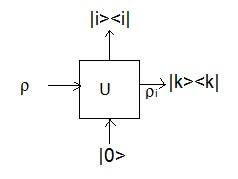
\includegraphics[scale=0.5]{immagini/von-neumann.jpg} %immagine
\end{center}
Prendiamo uno stato misto generico iniziale $\rho$ che interagisce mediante una trasformazione unitaria con un sistema ancillare, che prepariamo in un sistema di riferimento zero e che gioca il ruolo di pointer.\\
Nell'esperimento di Stern e Gerlach il sistema rappresenta lo spin e l'ancilla è il grado orbitale; mentre nel paradosso di Schrödinger il sistema è la particella che decade e l'ancilla è il gatto.\\
Si misura poi un'osservabile i che è associata ad un set ortonormale $\{\left|i\right\rangle\}$ tale che $I=\sum_{i}\left|i\right\rangle\left\langle i\right|$.
All'uscita il sistema entra in un nuovo apparato di misura dove facciamo un'altra misura sul sistema chiamata $\left|k\right\rangle\left\langle k\right|$, associata ad un altro set ortonormale $\{\left|k\right\rangle\}$ tale che $I=\sum_{k}\left|k\right\rangle\left\langle k\right|$.
Calcoliamo la probabilità congiunta di vedere il risultato $i$ sull'ancilla e il risultato $k$ nella misura fatta sul sistema:
\begin{equation}\begin{split}
p(i,k)=tr[\left|k\right\rangle\left\langle k \right|\otimes\left|i\right\rangle\left\langle i \right| U (\rho\otimes \left|0\right\rangle\left\langle 0\right|)U^+]
\end{split}\end{equation}
(utilizzando la regola di Born e la Schrödinger picture). \\
Si calcola poi la probabilità marginale di vedere i indipendentemente da ciò che si vede dopo:
\begin{equation}\begin{split}
p(i)=\sum_{k}p(1,k)=tr[I\otimes \left|i\right\rangle \left\langle i\right| U (\rho\otimes \left|0\right\rangle\left\langle 0\right|) U^+]
\end{split}\end{equation}
Calcoliamo la probabilità condizionata di vedere k se abbiamo visto i (con la formula di Bayes):
\begin{equation}\begin{split}
p(k|i)=\frac{p(i,k)}{p(i)}
\end{split}\end{equation}
All'uscita della prima misura il sistema si trova in uno stato $\rho_{i}$ tale che:
\begin{equation}\begin{split}
tr[\rho_{i}\left|k\right\rangle\left\langle k\right|]=p(k|i)
\end{split}\end{equation}
ricavo $\rho_{i}$:
\begin{equation}\begin{split}
p(k|i)=\frac{p(i,k)}{p(i)}=\\
\frac{tr[\left|k\right\rangle\left\langle k\right| tr_{2}[(I\otimes\left|i\right\rangle\left\langle i\right|)U(\rho\otimes\left|0\right\rangle\left\langle 0\right|)U^+]]}{tr[(I\otimes\left|i\right\rangle\left\langle i\right|) U (\rho\otimes\left|0\right\rangle\left\langle 0\right|)U^+]}
\end{split}\end{equation}
sappiamo che la traccia parziale di un operatore (R) si calcola come somma su\\un set ortonormale di:
\begin{equation}\begin{split}
tr_{2}[R]= \sum_{i}(I\otimes\left\langle i\right|)R(I\otimes\left|i\right\rangle)
\end{split}\end{equation}
utilizzando l'invarianza della traccia per permutazione ciclica e le decomposizioni $I\otimes\left|i\right\rangle\left\langle i\right|=(I\otimes\left|i\right\rangle)(I\otimes\left\langle i\right|)$  $\rho\otimes\left|0\right\rangle\left\langle 0\right|=(\rho\otimes I)(I\otimes\left|0\right\rangle)(I\otimes\left\langle0\right|)$ otteniamo:
\begin{equation}\begin{split}
tr_{2}[(I\otimes\left|i\right\rangle\left\langle i\right|)U(\rho\otimes\left|0\right\rangle\left\langle 0\right|)U^+]=\\
=(I\otimes\left\langle i\right|)U(I\otimes\left|0\right\rangle)\rho(I\otimes\left\langle 0\right|)U^+(I\otimes\left|i\right\rangle)= \\
=A_{i}\rho A_{i}^+
\end{split}\end{equation}
con $A_{i}=(I\otimes\left\langle i\right|)U(I\otimes\left|0\right\rangle)$ dove:
$(I\otimes\left\langle i\right|)$ rappresenta l'osservabile che misuriamo sul pointer, $U$ l'interazione unitaria tra sistema e ancilla, $(I\otimes\left|0\right\rangle)$ la preparazione del pointer/dell'ancilla cioè lo $z_{0}$ delle particelle. \\
Si ricava quindi:
\begin{equation}\begin{split}
\rho_{i}=\frac{A_{i}\rho A_{i}^+}{tr[A_{i}\rho A_{i}^+]}
\end{split}\end{equation}
che rappresenta lo stato che esce dall'apparato di misura dopo che ho letto il risultato, uno stato condizionato dalla conoscenza del risultato della misura precedente. \\
Abbiamo ottenuto questa relazione solamente utilizzando la regola di Born e rompendo lo stato entangled con Von Neumann.\\
Alla fine dell'interazione tra stato e misura, lo stato non è entangled ma resta solo una mistura tra gli stati che corrispondono ai due possibili risultati (stati che so calcolare).